% Contents of src/core/Math/StatisticalTests and their dependencies. Paper: section "Statistical tests"
% (fig:stattests); Doxygen: StatisticalTests.hpp.
%   pdflatex StatisticalTestsClasses.tex; pdftoppm -r 200 -png -singlefile StatisticalTestsClasses.pdf StatisticalTestsClasses;
%   pdftocairo -svg StatisticalTestsClasses.pdf StatisticalTestsClasses.svg
\documentclass[tikz,border=2pt]{standalone}
% Shared style of the class diagrams of CAP (figures/*Classes.tex): \input after \documentclass[tikz]{standalone}.
%  - boxes: blue = abstract base class, light blue = class, green = entry class of the folder (steering class, task),
%    yellow = free functions (tools), grey = class of another folder;
%  - arrows: open triangle = inherits from; dashed with diamond = owns (holds); dashed with arrow = uses.
\usepackage[scaled=0.92]{helvet}
\usetikzlibrary{arrows.meta,shapes.multipart,positioning,fit,backgrounds,calc}
\renewcommand{\familydefault}{\sfdefault}
\definecolor{abstract}{HTML}{D6E4F5}
\definecolor{concrete}{HTML}{EEF4FB}
\definecolor{steer}{HTML}{DCEFD9}
\definecolor{tools}{HTML}{FFF8E6}
\definecolor{external}{HTML}{E9E9E9}
\definecolor{dependline}{HTML}{8A6D3B}
\definecolor{folder}{HTML}{F7F7F7}
\tikzset{
  every picture/.style={font=\scriptsize},
  cls/.style={draw, fill=concrete, align=center, inner sep=2.5pt, text width=#1, font=\tiny},
  cls/.default=3.0cm,
  abs/.style={cls=#1, fill=abstract},
  abs/.default=3.0cm,
  steer/.style={cls=#1, fill=steer, line width=0.8pt},
  steer/.default=4.2cm,
  tool/.style={cls=#1, fill=tools},
  tool/.default=4.2cm,
  ext/.style={cls=#1, fill=external, dashed},
  ext/.default=2.6cm,
  fam/.style={draw, rectangle split, rectangle split parts=2, rectangle split part fill={#1,white},
              rectangle split part align={center,left}, inner sep=2.5pt, align=left},
  inherit/.style={-{Triangle[open,length=2.2mm,width=2.2mm]}, thin},
  uses/.style={dashed, dependline, -{Stealth[length=1.6mm]}, thin},
  owns/.style={dashed, dependline, {Diamond[length=2.4mm,width=1.6mm]}-, thin},
  lbl/.style={font=\tiny, text=dependline, align=center},
  note/.style={font=\tiny, align=left, text=black!70},
  title/.style={font=\footnotesize\bfseries, anchor=north west},
}
% a member line in a class box
\newcommand{\m}[1]{\\#1}
\newcommand{\cn}[1]{{\scriptsize\textbf{#1}}}
\newcommand{\an}[1]{{\scriptsize\textbf{\textit{#1}}}}

% legend common to the class diagrams (place with \legendat{x}{y})
\newcommand{\legendat}[2]{%
  \begin{scope}[shift={(#1,#2)}, font=\tiny]
    \node[abs=0.9cm, minimum height=3mm, inner sep=1pt] (lA) at (0,0) {abstract};
    \node[cls=0.9cm, minimum height=3mm, inner sep=1pt, right=1mm of lA] (lC) {class};
    \node[steer=1.1cm, minimum height=3mm, inner sep=1pt, right=1mm of lC] (lS) {entry class};
    \node[tool=1.1cm, minimum height=3mm, inner sep=1pt, right=1mm of lS] (lT) {functions};
    \node[ext=1.3cm, minimum height=3mm, inner sep=1pt, right=1mm of lT] (lE) {other folder};
    \draw[inherit] ($(lE.east)+(1mm,0)$) -- ++(5mm,0) node[right, inner sep=1pt] (l1) {inherits};
    \draw[owns] ($(l1.east)+(1mm,0)$) -- ++(5mm,0) node[right, inner sep=1pt] (l2) {owns};
    \draw[uses] ($(l2.east)+(1mm,0)$) -- ++(5mm,0) node[right, inner sep=1pt] {uses};
  \end{scope}}

\begin{document}
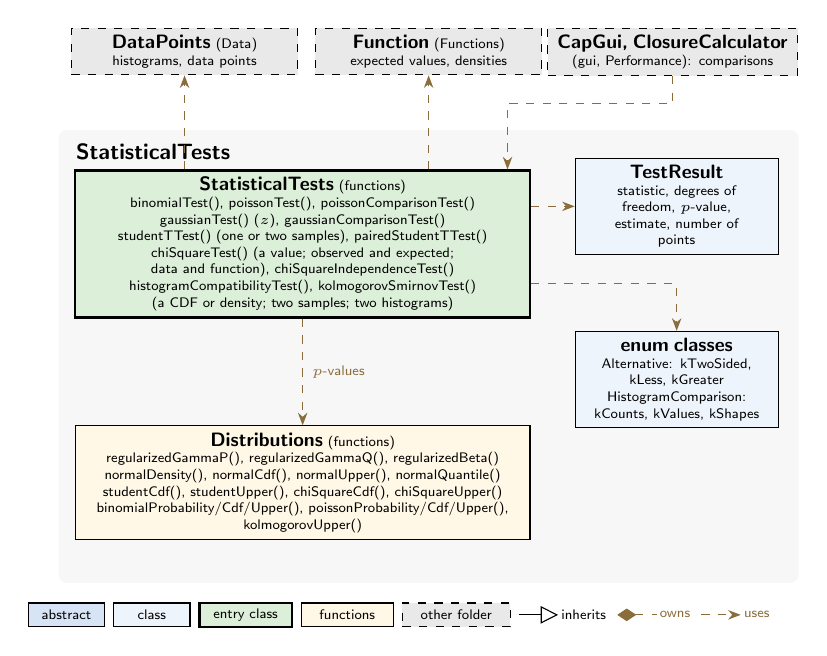
\begin{tikzpicture}[every node/.append style={anchor=north}]
  \begin{scope}[on background layer]
    \fill[folder, rounded corners=3pt] (-0.1,-1.0) rectangle (9.3,-6.75);
  \end{scope}
  \node[title] at (0.0,-1.05) {StatisticalTests};

  \node[ext=2.7cm] (DP) at (1.5,0.3) {\cn{DataPoints} \tiny(Data)\m{histograms, data points}};
  \node[ext=2.7cm] (PF) at (4.6,0.3) {\an{Function} \tiny(Functions)\m{expected values, densities}};
  \node[ext=3.0cm] (Gui) at (7.7,0.3) {\cn{CapGui, ClosureCalculator}\m{(gui, Performance): comparisons}};

  \node[steer=5.6cm] (Tests) at (3.0,-1.5)
    {\cn{StatisticalTests} \tiny(functions)\m{binomialTest(), poissonTest(), poissonComparisonTest()}
     \m{gaussianTest() ($z$), gaussianComparisonTest()}
     \m{studentTTest() (one or two samples), pairedStudentTTest()}
     \m{chiSquareTest() (a value; observed and expected;}\m{data and function), chiSquareIndependenceTest()}
     \m{histogramCompatibilityTest(), kolmogorovSmirnovTest()}\m{(a CDF or density; two samples; two histograms)}};
  \node[cls=2.4cm] (TR) at (7.75,-1.35)
    {\cn{TestResult}\m{statistic, degrees of}\m{freedom, $p$-value,}\m{estimate, number of}\m{points}};
  \node[cls=2.4cm] (Enums) at (7.75,-3.55)
    {\cn{enum classes}\m{Alternative: kTwoSided,}\m{kLess, kGreater}\m{HistogramComparison:}\m{kCounts, kValues, kShapes}};
  \node[tool=5.6cm] (Dist) at (3.0,-4.75)
    {\cn{Distributions} \tiny(functions)\m{regularizedGammaP(), regularizedGammaQ(), regularizedBeta()}
     \m{normalDensity(), normalCdf(), normalUpper(), normalQuantile()}
     \m{studentCdf(), studentUpper(), chiSquareCdf(), chiSquareUpper()}
     \m{binomialProbability/Cdf/Upper(), poissonProbability/Cdf/Upper(),}\m{kolmogorovUpper()}};

  \draw[uses] (Tests.east |- TR.west) -- (TR.west);
  \draw[uses] (Tests.east |- 0,-2.95) -| (Enums.north);
  \draw[uses] (Tests.south) -- node[lbl, right]{$p$-values} (Dist.north);
  \draw[uses] (1.5,0 |- Tests.north) -- (DP.south);
  \draw[uses] (4.6,0 |- Tests.north) -- (PF.south);
  \draw[uses] (Gui.south) -- ++(0,-0.35) -| ([xshift=-0.3cm]Tests.north east);
  \legendat{0.0}{-7.0}
\end{tikzpicture}
\end{document}
